\documentclass{beamer}

\usepackage{lmodern}
\usepackage[french]{babel}
\usepackage[utf8]{inputenc}
\usepackage[T1]{fontenc}
\usepackage{makecell}


\usetheme{Warsaw}
\setbeamerfont{page number in head/foot}{size=\large}

\beamertemplatenavigationsymbolsempty
\date{}
\author{Arthur Burgada \and Pierre-Hugues Blelly}

\title{Détection des ondes gravitationnelles}
\begin{document}

\begin{frame}
	\titlepage
\end{frame}

\begin{frame}
	\frametitle{Plan de l'exposé}
	\tableofcontents
\end{frame}

\section{Les ondes gravitationnelles}
\begin{frame}
	\frametitle{Découverte théorique}
	\begin{itemize}
		\item 1916 : Relativité Générale de Einstein
		\item En linéarisant les équations un terme d'onde progressive apparaît
		\item Artefact mathématique ou réalité physique ?
	\end{itemize}
\end{frame}

\begin{frame}
	\begin{itemize}
		\item Analogue à onde électromagnétique : émis lorsque un corps massique accélère
		\item Vitesse de propagation c
		\item Mais décroissance en 1/R
		\item Amplitude extrêmement faible
		\bigskip
		\center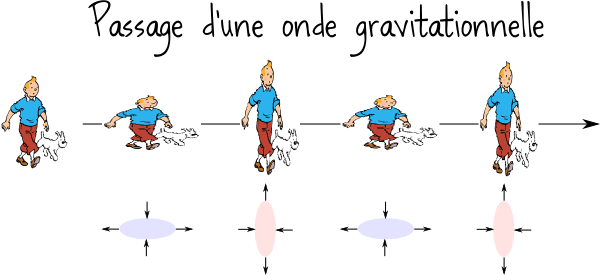
\includegraphics[scale = 0.4]{Docs/tintin.png}
	\end{itemize}

\end{frame}


\begin{frame}
	\frametitle{Mise en évidence indirecte : Pulsar de Hulse et Taylor}
	\begin{columns}
	\begin{column}{0.5\textwidth}
		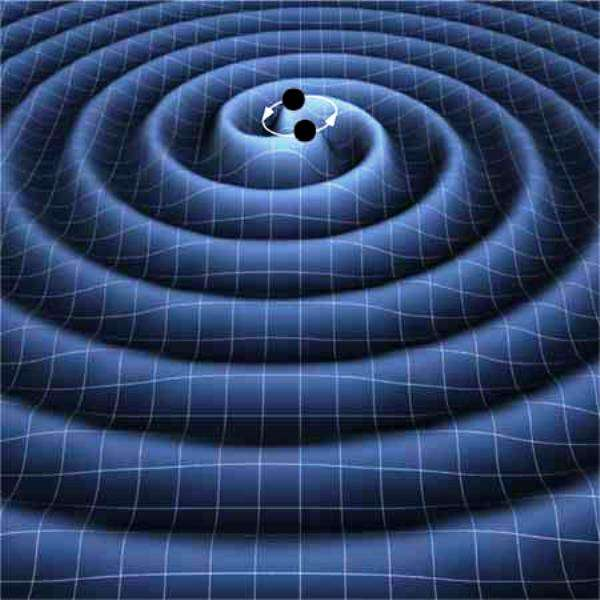
\includegraphics[scale=0.2]{Docs/pulsar_binaire.jpeg}
	\end{column}
	\begin{column}{0.5\textwidth}
	\begin{itemize}
		\item Couple de 2 étoiles dont l'une est une étoile à neutrons
		\item PSR B1913+16 découvert en 1974
	\end{itemize}
	\end{column}
	\end{columns}
\end{frame}

\begin{frame}
	\frametitle{Mise en évidence indirecte : Pulsar de Hulse et Taylor}
	\begin{columns}
	\begin{column}{0.5\textwidth}
		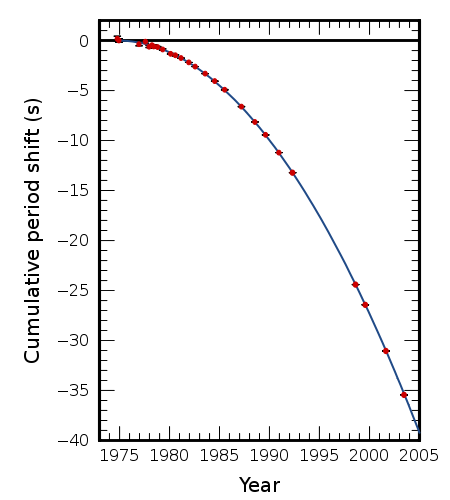
\includegraphics[scale=0.3]{Docs/period_shift_pulsar.png}
	\end{column}
	\begin{column}{0.5\textwidth}
		\begin{itemize}
			\item Période de 7,75 heures
			\item Diminution de la période dûe à l'émission d'ondes gravitationnelles
		\end{itemize}

	\end{column}
	\end{columns}
\end{frame}

\begin{frame}
	\frametitle{Enjeux du projet LIGO/VIRGO}
	\begin{itemize}
		\item Mise en évidence directe
		\item Précision suffisante
		\item Evaluer le taux d'expansion de l'Univers de manière indépendante de la technique utilisant la luminosité des supernovas
	\end{itemize}

\end{frame}


\section{Présentation du Michelson}

\begin{frame}
	\frametitle{Interféromètre de Michelson}
	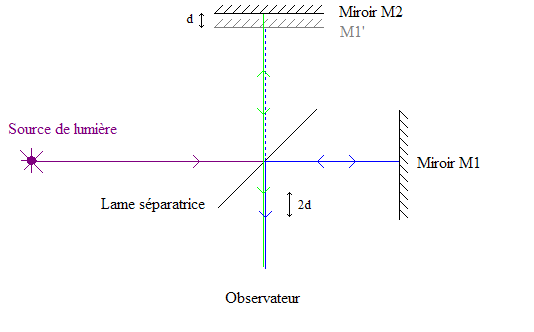
\includegraphics[scale=0.5]{Docs/interferometre_michelson.png}
\end{frame}


\begin{frame}
	\frametitle{Principe de la détection}
	\begin{columns}
		\begin{column}{0.5\textwidth}
			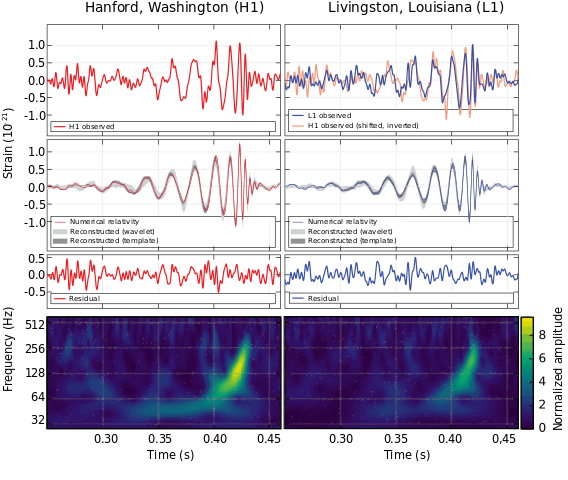
\includegraphics[width=\textwidth]{Docs/detection.png}		
		\end{column}
		\begin{column}{0.5\textwidth}
			Distortion de l'espace-temps
			\\
			On détecte cette distortion grâce à un interféromètre
		\end{column}
	\end{columns}
\end{frame}
\section{Présentation des interféromètres LIGO / VIRGO}
\begin{frame}
	\frametitle{L'interféromètre VIRGO}
	\begin{columns}
		\begin{column}{0.5\textwidth}
			\small
			\begin{enumerate}[-]
				\item 2 bras de 4km de long parfaitement horizontaux (Sous vide)
				\item Un système optique  totalement isolé de l'exterieur
			\end{enumerate}
		\end{column}
		\begin{column}{0.5\textwidth}
			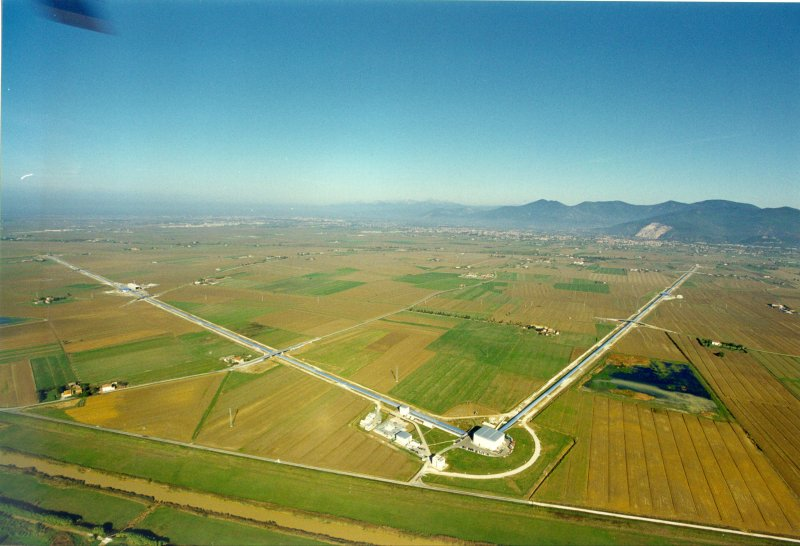
\includegraphics[scale=.5]{Docs/virgoview.png}
		\end{column}
	\end{columns}
	\bigskip
	3 interféromètres: VIRGO (Italie) et LIGO(Hanford(Washington) / Livinston (Louisianne))
\end{frame}
\section{LASER utilisés}

\begin{frame}
	\frametitle{Système à injection}
	\begin{columns}
		\begin{column}{0.5\textwidth}
			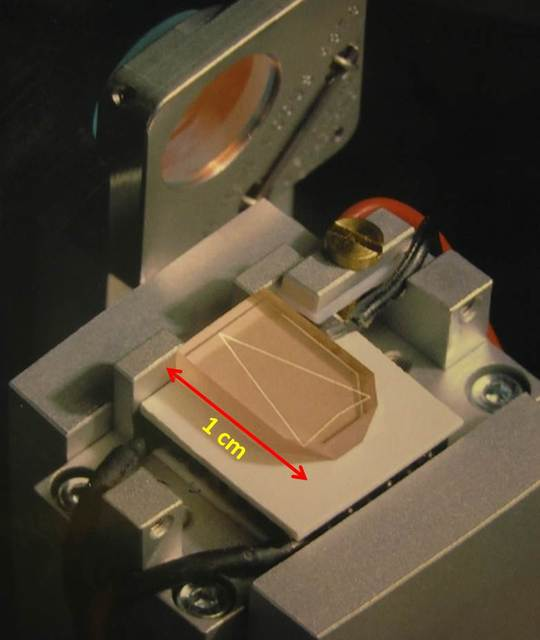
\includegraphics[width=\textwidth]{Docs/NPRO.png}
		\end{column}
			

		\begin{column}{0.5\textwidth}
				\begin{itemize}
					\item 2 Lasers: Un laser maître et un laser esclave
					\item On injecte un rayonnement laser dans la cavité du second laser pour faire changer son gain et modifier la fréquence d'émission du second laser.
				\end{itemize}
		\end{column}
	\end{columns}
\end{frame}



\begin{frame}
	\frametitle{Le laser de VIRGO}
	Fonctionne en deux étapes
	\begin{enumerate}[1.]
		\item Emission du laser Maître
		\item Emission du laser Esclave 
	\end{enumerate}
	\begin{table}
	\small
	\centering
	\begin{tabular}{|l|l|l|}
	\hline
		\thead{Taille du faisceau \\ ($W_0$ [mm])}& \thead{Longueur de Rayleigh \\ ($z_0$ [m])} & \thead{Divergence du \\ faisceau ($\theta_0$ [$\mu rad$])} \\
		\hline
		4.5 +/- 0.5 & 60 +/- 10 & 75 -/+ 10 \\
		\hline
	\end{tabular}
	\end{table}

\end{frame}
\begin{frame}
\frametitle{Le laser LIGO}
Fonctionnement en quatre étapes:
\begin{itemize}
	\item Emission du laser maître
	\item Emission du laser esclave
	\item Première amplification
	\item Seconde amplification
\end{itemize}
\end{frame}

\section{Cavités de Fabry-Pérot}


\section{Cavité de recyclage}
\begin{frame}
	\frametitle{Cavité de Recyclage}
	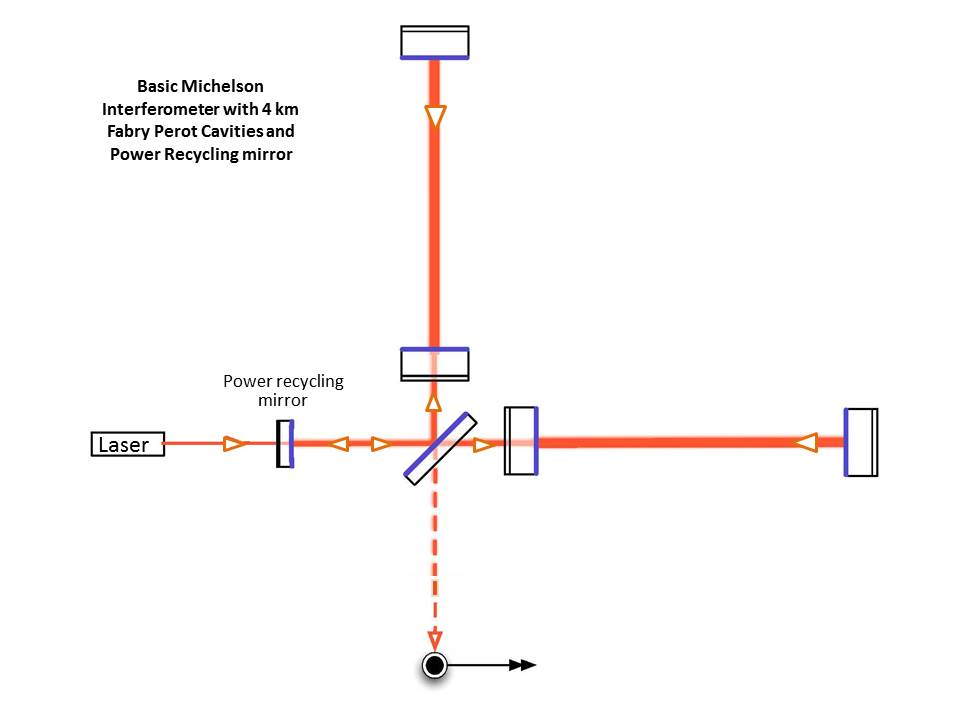
\includegraphics[height=\textheight]{Docs/recycling_mirrors.png}
\end{frame}

\begin{frame}
	\frametitle{Les Miroirs}
	\begin{columns}
	
		\begin{column}{0.5\textwidth}
			\begin{itemize}
				\item Miroirs en silice
				\item Pertes très faibles ( < 2\%)
				\item Abbérations ($10^{-8} m$)
				\item Diamètre: 35 cm
			\end{itemize}
		\end{column}
		
		\begin{column}{0.5\textwidth}
			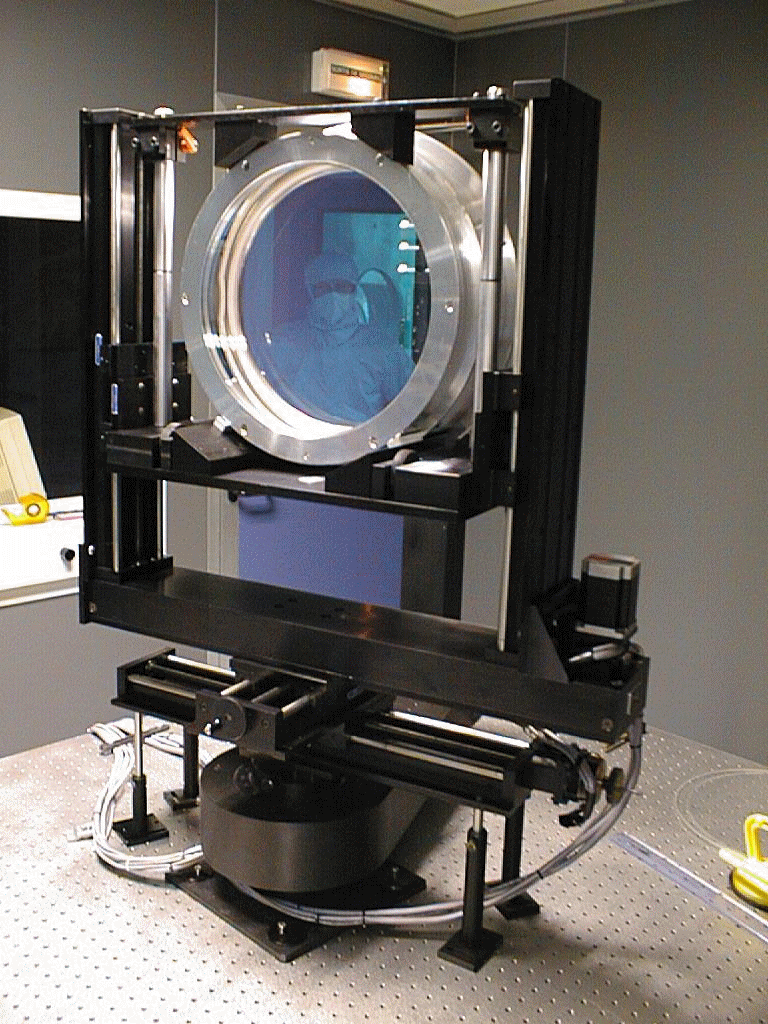
\includegraphics[width=\textwidth]{Docs/miroir.png}
		\end{column}
	\end{columns}
\end{frame}

\end{document}
